\chapter{Discussion: Where and Why Reconstruction Fails}
\label{ch:discussion}

\section{Answers to the Research Questions}
\paragraph{RQ1: does GoT beat CoT and ToT on stage recall?} Not reliably. GoT's mean stage recall is highest in most settings, but only 2 of 15 paired comparisons are below $p=0.05$ before correction and none survives it (Table~\ref{tab:tests}), so H0 is not rejected for the primary metric. GoT does show a more consistent advantage in event recall (uncorrected $p<0.05$ in 5 of 10 comparisons), paid for with lower precision at 7B--8B. Three seeds per cell and the pairing of seeds as observations limit what can be concluded.
\paragraph{RQ2: where does reconstruction fail, and what changes the numbers?} Four failure modes explain most of the loss, described below. The interventions that worked address them directly: stage definitions address labelling, triage addresses noise, and a larger model addresses detection and labelling together.
\paragraph{RQ3: does a security-tuned model change the conclusion?} No. Llama-Primus-Reasoning was significantly worse than Llama 3.1 8B on identical evidence, partly through output-format failures, and no topology comparison was significant for it.

\section{Failure 1: Most Attack Events Are Never Detected}
Reading outputs against ground truth, only 15.3\% of the 89 true events are ever reported, regardless of topology. The attack is a small fraction of each graph (2.6\% of nodes in WS12, 5.9\% in APT29), and many of its steps use ordinary administrative utilities that look benign without attacker context. A method cannot aggregate evidence that no step flagged. This also bounds every recall figure in Chapter~\ref{ch:results}.

\section{Failure 2: Stage Labels Are Miscalibrated}
Among the events that are found, exact stage accuracy is about 20\%, against 10\% for a random choice among ten stage names. Each model has a stable preference over stage names that does not match this data. Qwen 2.5 7B assigns Initial Access to only 3.9\% of the events it reports and Lateral Movement to 1.1\%, whereas those two stages are 8 of the 14 (57\%) ground-truth events of WS12 and Ubuntu together. This explains Qwen's exact stage recall of 0.000 under CoT and ToT. Figures~\ref{fig:conf-llama} and~\ref{fig:conf-qwen} show where predicted and true stages disagree.

\begin{figure}[H]
\centering
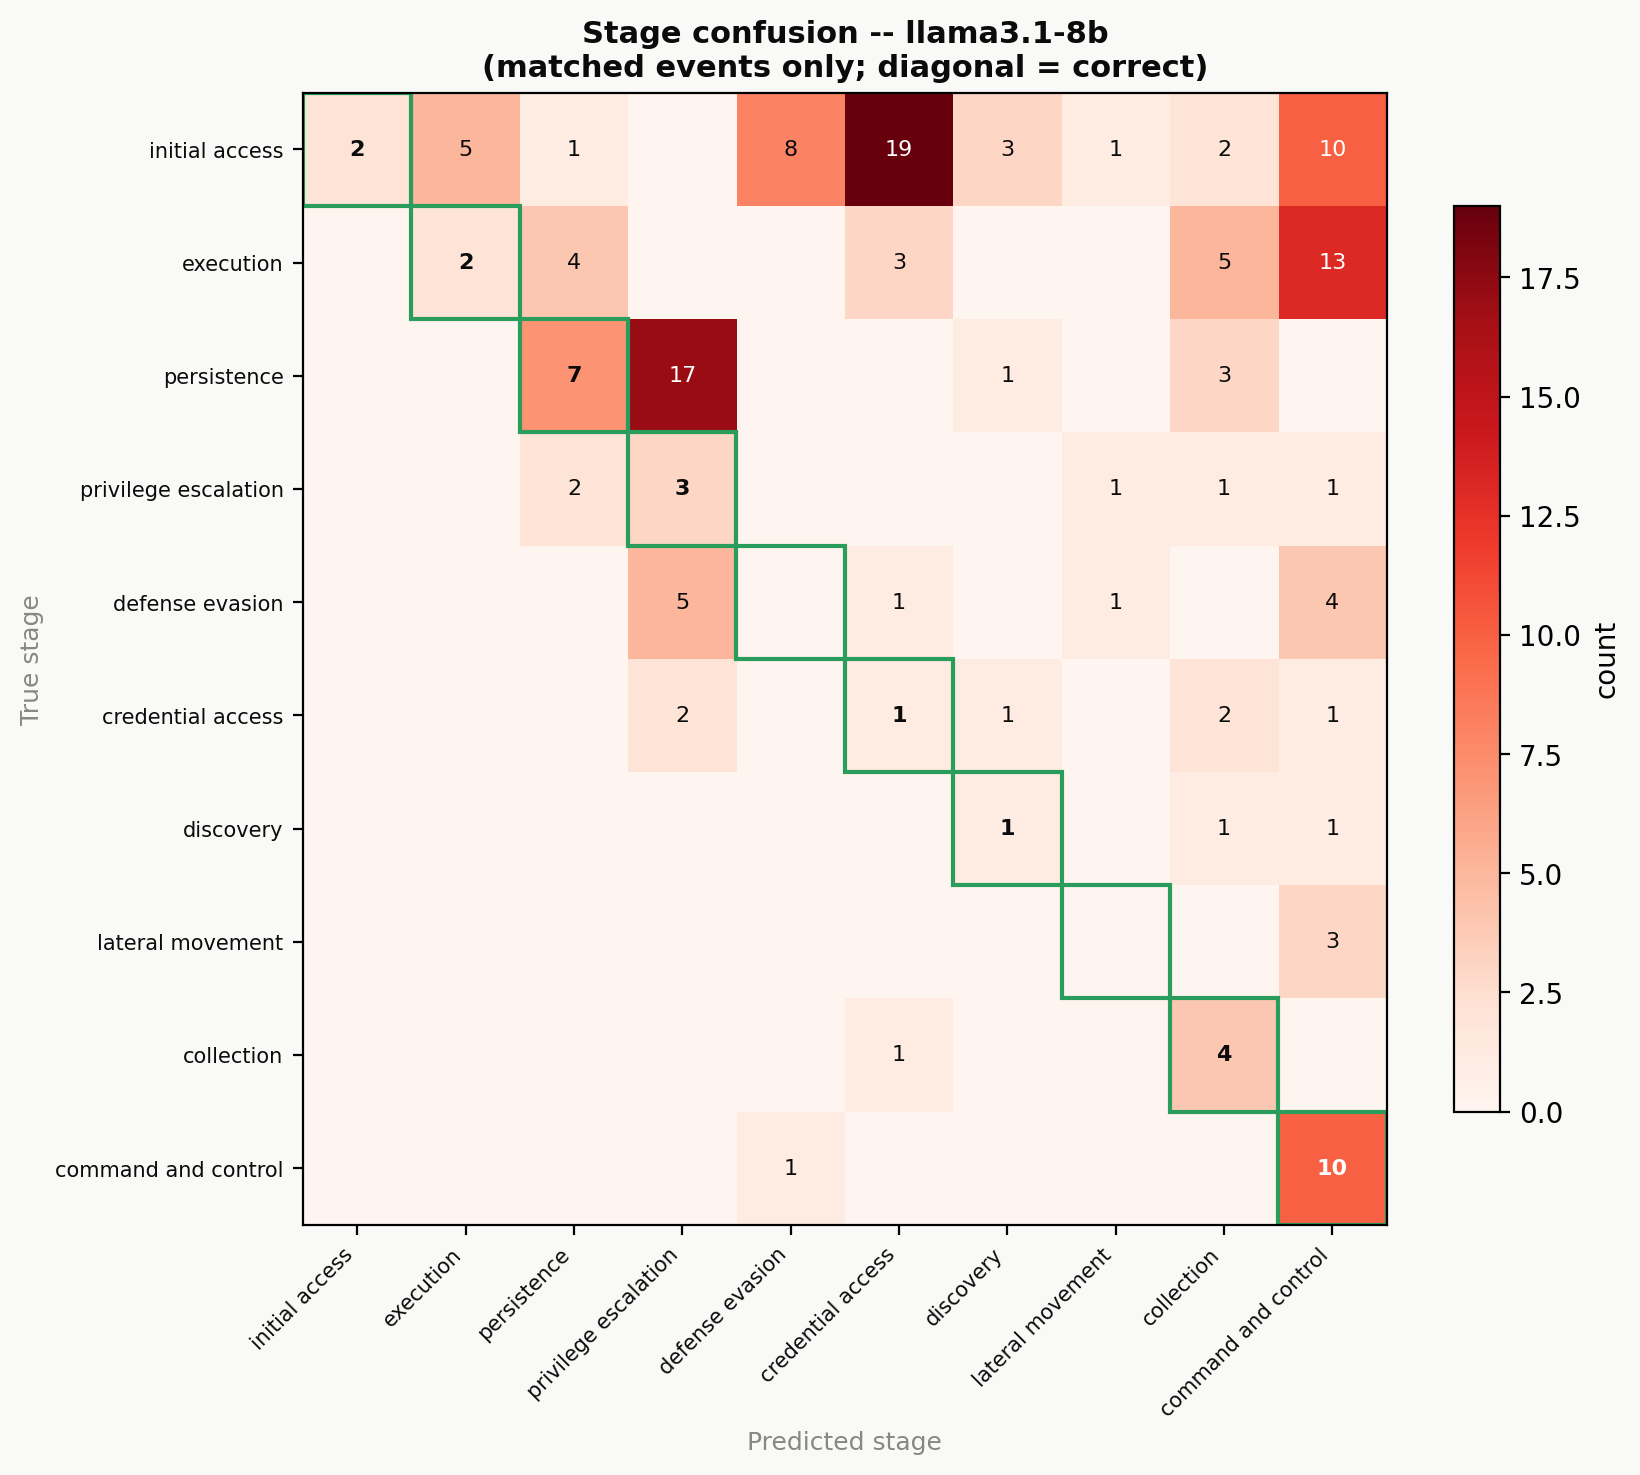
\includegraphics[width=0.8\textwidth]{fig_confusion_llama8b}
\caption{Stage confusion matrix for Llama 3.1 8B: true stage against predicted stage over all found events.}
\label{fig:conf-llama}
\end{figure}

\begin{figure}[H]
\centering
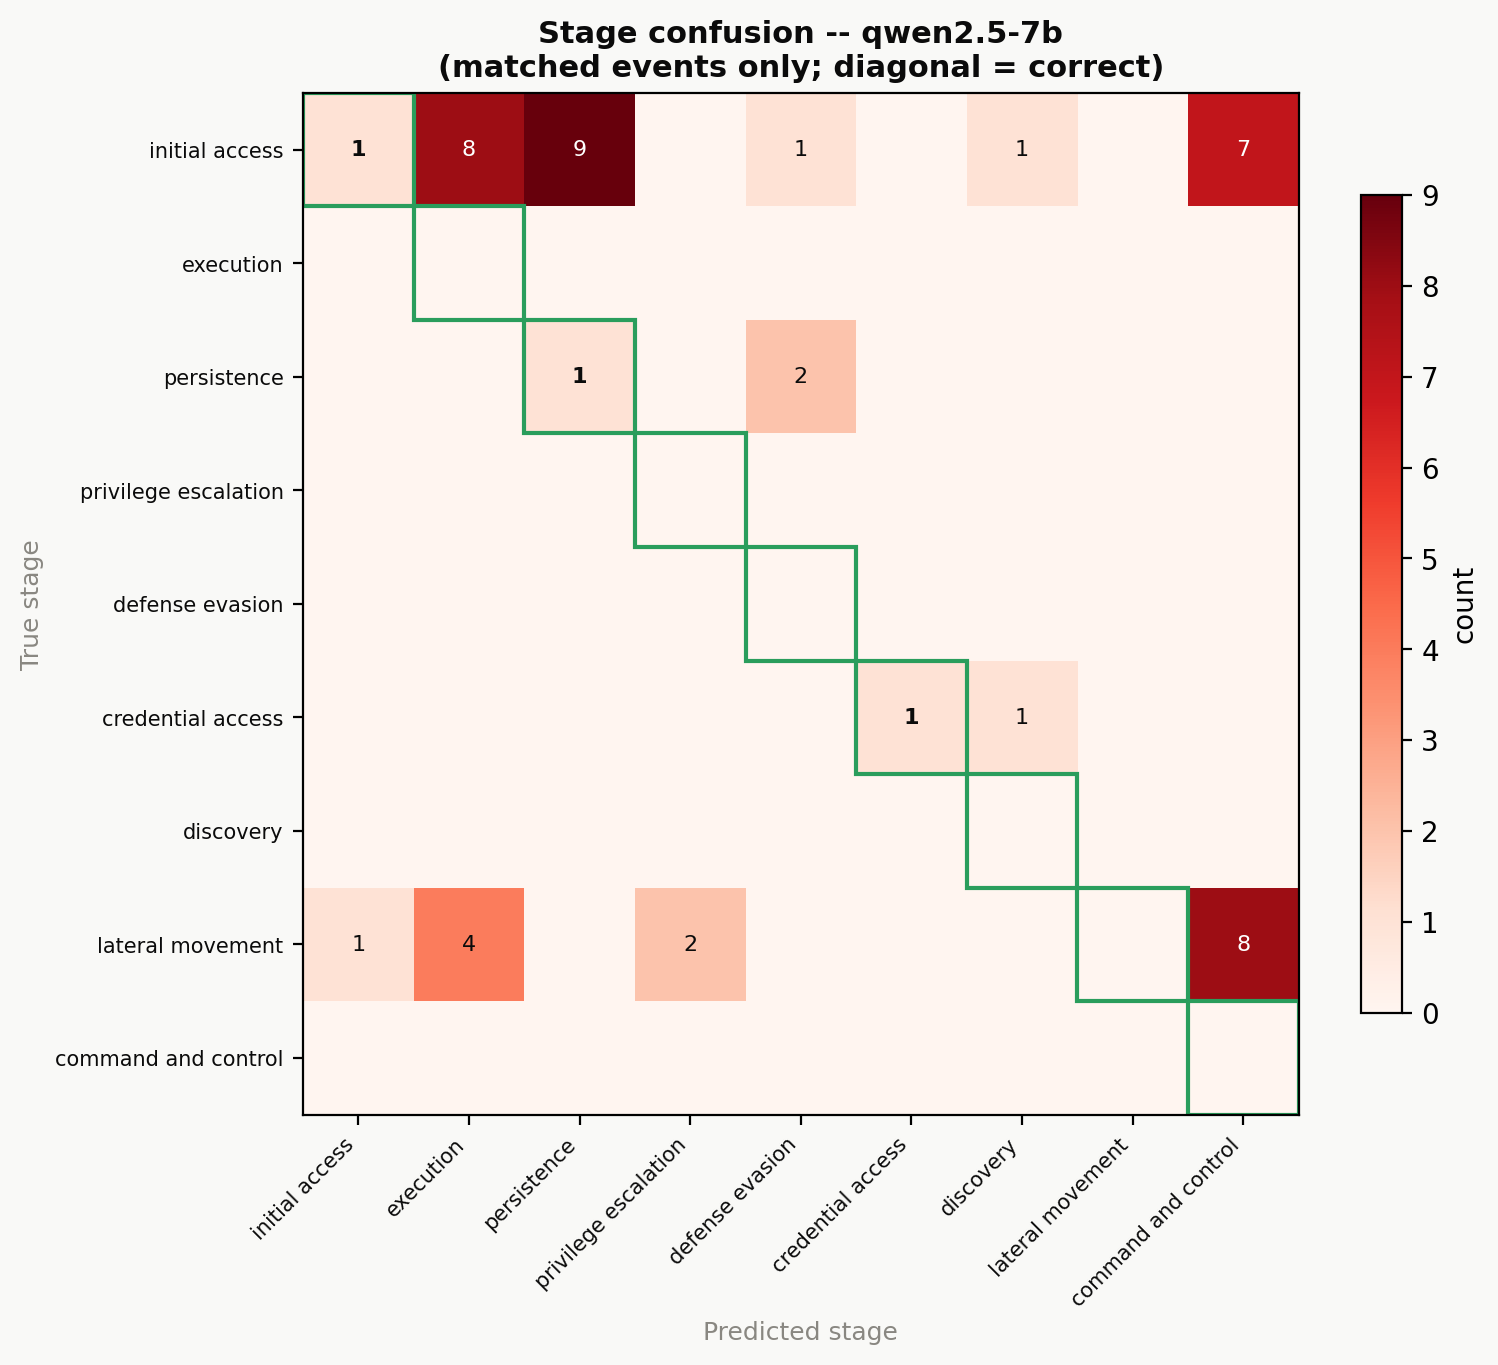
\includegraphics[width=0.8\textwidth]{fig_confusion_qwen7b}
\caption{Stage confusion matrix for Qwen 2.5 7B.}
\label{fig:conf-qwen}
\end{figure}

The fix that worked was to supply the vocabulary: adding stage definitions to the prompt doubled exact stage recall (Section~\ref{sec:res-rounds}).

\section{Failure 3: Evidence the Method Cannot Use or Cannot Tell Apart}
\subsection{The Shared Windows 10 Log}
Sidewinder, FIN6 and APT29 share one evidence file, so the model sees the same 624 nodes whichever attack it is asked about. All three score far below WS12 and Ubuntu (Figure~\ref{fig:heatmap}) and Primus scores zero on Sidewinder. This is a limit of the data, not of any topology.

\subsection{Why the Aggregate Mechanism Did Not Show}
\label{sec:disc-mechanism}
The argument for H1 needs two things: attack events must be spread across segments, and each segment's analysis must retain its part. Neither is well supported here.
\begin{enumerate}
\item \textbf{Low per-segment detection.} With only 15.3\% of true events detected at all, the per-segment results rarely contain the pieces to be merged.
\item \textbf{Little scattered structure in the data.} A pre-check on WS12 found that all attack events fall into one segment after balanced splitting. Aggregate then has nothing to link, and GoT reduces to analysing one segment and restating it.
\item \textbf{Aggregation loses information.} The merge call sees only the per-segment answers, not the evidence behind them, so an event omitted from a segment answer cannot be recovered at that step.
\end{enumerate}
The v5 variant, which gives Aggregate the cross-segment links explicitly, raised GoT's scores but not significantly. That fits a mechanism that works in principle but is starved of inputs.

\section{Failure 4: Input Length and Output Format}
\subsection{Input Length}
The Llama 70B comparison shows that the same model can be strong or weak depending on input length alone (Figure~\ref{fig:length}). On the 16--19K-token inputs it beats the 8B (precision 0.44 against 0.30); on the 58K-token inputs its recall collapses to 0.09 (8B: 0.22). Triage shortens the input and helps; so, plausibly, does GoT's segmentation, because most of its calls read a quarter of the evidence. GoT's consistent advantage in event recall, with lower precision, is what shorter, independent per-segment reads would produce, so it could come from splitting rather than aggregating. A segmented-CoT control, with the same split and a plain concatenation of the segment answers instead of an LLM merge, would separate the two. We did not run it.

\subsection{Output Format}
For the security-tuned model, 38\% of runs ended without a parseable answer (Figure~\ref{fig:parse}). With constrained decoding off, a long reasoning trace can consume the output budget before any JSON is written. This is a pipeline limitation as much as a model one, which is why we do not read the Primus result as evidence against security tuning in general.

\section{Failure 5: Unannotated Activity Counts as an Error}
All methods independently report a second command chain in WS12 that is not in the annotation. We checked it against the official attack description and it is real activity, so some false positives are genuinely correct findings. They lower precision about equally for all methods, so they do not bias the topology comparison, but they make absolute precision values conservative.

\section{Status of the Claims}
\begin{table}[H]
\centering
\caption{What the evidence supports.}
\label{tab:claims}
\small
\begin{tabularx}{\textwidth}{@{}>{\raggedright\arraybackslash}p{5.3cm} >{\raggedright\arraybackslash}p{2.9cm} Y@{}}
\toprule
\textbf{Claim} & \textbf{Status} & \textbf{Evidence} \\
\midrule
GoT beats CoT and ToT on stage recall & Not supported & 2 of 15 uncorrected $p<0.05$; none after correction \\
GoT gives higher event recall & Suggestive & 5 of 10 uncorrected $p<0.05$; none after correction; lower precision \\
Stage definitions raise stage recall & Supported & 0.056 to 0.123, $p=0.0015$ \\
Triage raises precision & Supported & 0.245 to 0.329, $p=0.04$ \\
Larger model raises stage recall (Qwen) & Supported & 0.15 to 0.30, $p=0.012$ \\
Long input hurts a large model & Supported (one comparison) & 70B recall 0.09 against 8B 0.22 at 58K tokens \\
Security tuning helps & Not supported & Primus F$_1$ 0.101 against 0.295, $p<0.001$ \\
GoT's gain is due to aggregation & Untested & Needs ablation and segmented-CoT control \\
\bottomrule
\end{tabularx}
\end{table}

\section{Threats to Validity}
\begin{itemize}
\item \textbf{Statistical power and pairing.} Three seeds per cell cannot detect small effects, and treating each seed of a scenario as a separate paired observation makes the tests anti-conservative. We report 30 topology tests without correction in the table and state which survive correction (none). A non-significant result means ``not shown'', not ``shown to be absent''.
\item \textbf{Few scenarios, one shared log.} Five scenarios, three of which share their evidence, are not five independent samples.
\item \textbf{Asymmetric grid.} Qwen 7B could run only the two short scenarios, so cross-model comparisons use WS12 and Ubuntu only.
\item \textbf{Substring matching.} A correct event described with different text would be counted as a miss, for every method equally.
\item \textbf{Model range.} Only models from 7B to 70B were tested, and one security-tuned model.
\end{itemize}

\section{What the Audit Taught Us}
The defects of Chapter~\ref{ch:audit} each had the potential to change the answer silently: a label-leaking field, overwritten nodes, an unbalanced split that gave one GoT segment most of the evidence, and a job that reported success after a crash. In a comparison of this kind, the engineering around the methods deserves as much scrutiny as the methods.
